\subsection*{Big Bridge}
"Let's see how you handle the mighty me! And by me, I mean Gilgamesh!! And by handle, I mean DIE!!!" \\
\indent -- Gilgamesh \\\\
\noindent
When departing from Cornelia and heading north, the party finds themselves in the forests and grasslands surrounding the city.
After several hours of travel through the quiet nature, they arrive at the Big Bride, which is massive but also old and brittle.
When they reach its end, they encounter Gilgamesh who seems to have been awaiting them.
Gilgamesh is not necessarily good or evil, he travels the world to find powerful weapons for his collection.
Garland has convinced Gilgamesh to work for him and lets him guard the bridge from anyone who tries to cross.
In return, Garland gifted him the legendary sword Excalibur or at least that is what Gilgamesh believes.
Upon meeting the party, Gilgamesh will recognize them as potentially worthy opponents and draw his weapons.
\pagebreak

\tcbox[left=0pt,top=0pt,right=0pt,bottom=0pt, boxsep=0pt, colframe=accent, sharp corners]{
	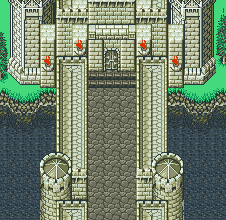
\includegraphics[width=0.96\columnwidth]{./art/maps/bridge.png} 
}

\subsubsection*{Battle on the Big Bridge}
The battle against Gilgamesh takes place at the end of the bridge as shown on the map above.
His combat details are shown below, but depending on the party you may need to modify some of his attributes.
When Gilgamesh is reduced to 0 HP he does not immediately faint, instead he finally pulls out Excalibur for one last attack.
He tries to attack the closest party member with it, but the sword deals no damage and immediately breaks.
Gilgamesh realizes that Garland has tricked him and seeing no other option, he flees. 
As he remains alive, the party may meet Gilgamesh again in the future.
After defeating Gilgamesh, the party can finally cross the bridge to reach the dark forest before the Chaos Shrine.
The forest is unusually quiet and most of its trees and plants seem to have died out.
The adventurers will very likely not be able to reach the Shrine before sunset, so they probably have to rest the night in the forest.

\vspace{0.5cm}

\monster{Gilgamesh}{2}{
\includegraphics[width=0.17\textwidth]{./art/monsters/gilgamesh.png}}
{
 PV: & \hfill 45 & PM: & \hfill 40\\
 FUE: & \hfill 2 & DEF: & \hfill 1 \\
 MAG: & \hfill 0 & RES: & \hfill 0 \\
 AGI: & \hfill 4 & Tamaño: & \hfill M\\
}
{
 \textbf{Arma de Asta}: 1d de daño \hfill \textbf{Botín}: 500 Gil 
 
 \mtech{Garra Letal}{6}{0t}{Único}{Arma}{
 Realiza dos \hyperlink{action}{Ataques} contra el objetivo. Si al menos uno de ellos lo golpea, queda \hyperlink{status}{Inmóvil} por 1 turno. }{\immobile} \mtech{Danza de Espadas}{8}{1t}{3u}{Tú}{Realiza un \hyperlink{action}{Ataque} contra todos los enemigos dentro del área de efecto.}{}
 \mreaction{Poder Crítico}{Cuando tus PV sean menos de 20, recibes \hyperlink{status}{aumFUE} hasta el final de la batalla.} 
}

\pagebreak